\documentclass{article}
\usepackage[margin=1in]{geometry}
\usepackage{amsmath,amsthm,amssymb}
\usepackage{bbm,enumerate,mathtools}
\usepackage{tikz,pgfplots}
\usepackage{chessboard}
\usepackage[hidelinks]{hyperref}
\usepackage{multicol} % Problem 35

\newenvironment{question}{\begin{trivlist}\item[\textbf{Question.}]}{\end{trivlist}}
\newenvironment{note}{\begin{trivlist}\item[\textbf{Note.}]}{\end{trivlist}}
\newenvironment{references}{\begin{trivlist}\item[\textbf{References.}]}{\end{trivlist}}
\newenvironment{related}{\begin{trivlist}\item[\textbf{Related.}]\end{trivlist}\begin{enumerate}}{\end{enumerate}}


\begin{document}

\rating{3}{3}
Suppose that Arthur chooses an arbitrary subset $A \subseteq [n]$, and Bri
attempts to discover it by repeatedly asking questions of the form,
``How many elements does $A$ have in common with $B_i \subseteq [n]$?''
\begin{figure}[ht!]
  \centering
  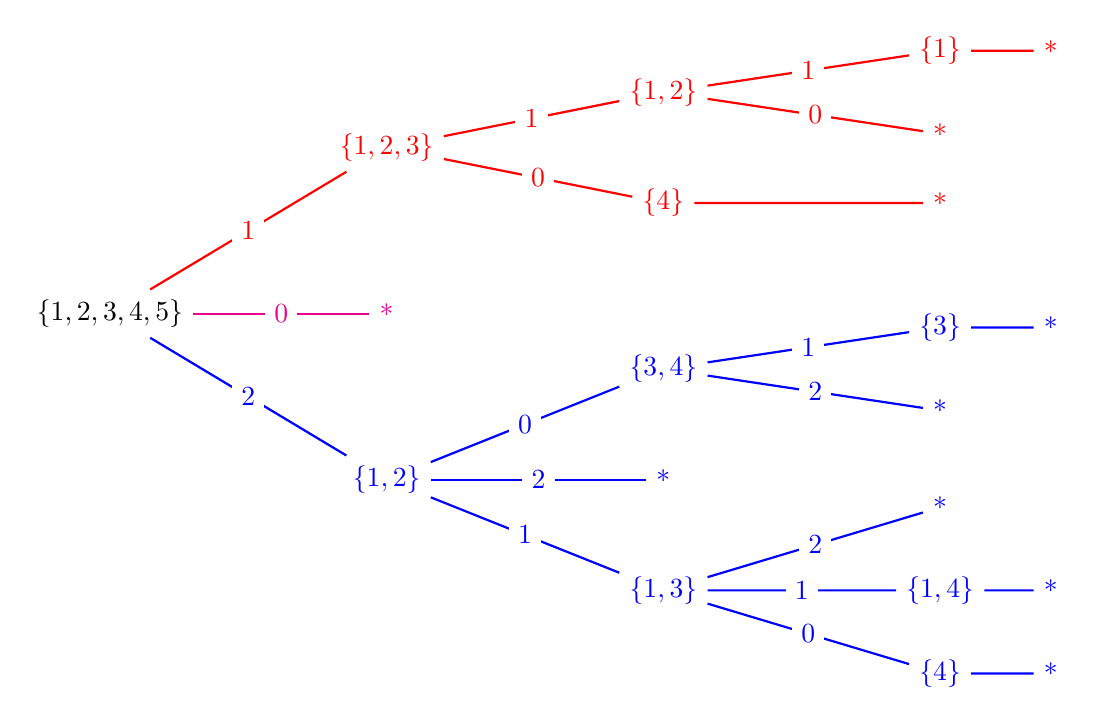
\begin{tikzpicture}[grow = right,
    thick,
    level 1/.style={sibling distance=6em,level distance=10em},
    level 2/.style={sibling distance=4em,level distance=10em},
    level 3/.style={sibling distance=3em,level distance=10em},
    level 4/.style={sibling distance=3em,level distance=4em},
  ]
  \node {$\{ 1,2,3,4,5 \}$}
    child[blue] {
      node {$\{ 1,2 \}$}
      child {
        node {$\{ 1,3 \}$}
        child {
          node {$\{ 4 \}$}
          child { node {*} }
          edge from parent node[fill=white] {0}
        }
        child {
          node {$\{ 1,4 \}$}
          child { node {*} }
          edge from parent node[fill=white] {1}
        }
        child {node {*} edge from parent node[fill=white] {2}}
        edge from parent node[fill=white] {1}
      }
      child {node {*} edge from parent node[fill=white] {2}}
      child {
        node { $\{ 3,4 \}$ }
        child {node {*} edge from parent node[fill=white] {2}}
        child {
          node {$\{ 3 \}$}
          child { node {*} }
          edge from parent node[fill=white] {1}
        }
        edge from parent node[fill=white] {0}
      }
      edge from parent node[fill=white] {2}
    }
    child[magenta] {
      node {*} edge from parent node[fill=white] {0}
    }
    child[red] {
      node {$\{ 1,2,3 \}$}
      child {
        node {$\{4\}$}
        child {
          node {*}
        }
        edge from parent node[fill=white] {0}
      }
      child {
        node {$\{1,2\}$}
        child { node {*} edge from parent node[fill=white] {0} }
        child {
          node {$\{1\}$}
          child { node {*}}
          edge from parent node[fill=white] {1}
        }
        edge from parent node[fill=white] {1}
      }
      edge from parent node[fill=white] {1}
    }
  ;
  \end{tikzpicture}
  \caption{A strategy that Bri can use to discover $A$ in four guesses or fewer,
  note that the cases where $A$ is size $3, 4,$ or $5$ follow by symmetry.}
\end{figure}

\begin{question}
  Let $a(n) = k$ be the least integer $k$ such that there exists a strategy
  where Bri can always determine $A$ in $k$ guesses or fewer. What is $a(n)$?
\end{question}

\begin{related}
  \item What if instead of giving the size of the intersection, Arthur gives the
  size of the symmetric difference?
  \item What if $A$ is a multiset?
  Where $i$ can occur with multiplicity at most $a_i$?
  \item What are some upper and lower bounds?
  \item How many (essentially different) optimal strategies exist? (e.g., do you always have to start by guessing the entire set?)
  \item What is the best \textit{average case} strategy?
  \item What if there are restrictions on Bri's subsets?
  For example, if the size of Bri's subsets must be weakly decreasing, or if
  Bri's subsets cannot simultaneously contain both $i$ and $i + 1$?
  \item What if Arthur instead picks a column from a given matrix, how many 
  questions of the form ``what is the $i$th entry'' does Bri have to ask in
  order to determine the column?
\end{related}

\begin{references}
  \item \url{https://math.stackexchange.com/a/25297/121988}
\end{references}
\end{document}
